% DISCUSSION  related to the reproducibility of this technique
\chapter{Discussion of Framework for Determing Resilience}

\section{Software Consideration}

The ease of providing data was a key design factor considered when designing the data collection method for this project. The goal was to create an online survey which could be done by the majority of participants in under 5 minutes, without missing out on potentially valuable data. This required a balancing act of maximising potential data gathered from a single participant against maximising number of participants. To do this several iterations were created and trialled.
\paragraph{}
Due to ease of later analysis, ease of repeatability, accessibility,  avoidance of disease spread and other major benefits an online survey method was chosen. The major downside of this technique is that it could exclude certain sectors of society due to lack of access to the internet. However, in Norway over 99 percent of the population have access to the internet (ssb https://www.ssb.no/en/statbank/table/11000/tableViewLayout1/ ) *MAYBE GO INTO MORE DETAIL HERE, E.G. SMARTPHONE ACCESS*
\paragraph{}
Once online surveys were the chosen method then which software was most appropriate needed to be considered. To do so many softwares were explored and then basic surveys were created and then tested on desktops, laptops, tablets, IOS smartphones and Android Smartphones on the perceived best candidates. The results of this exploration are outlined on table** below.

\begin{table}[!ht]
    \centering
    \begin{tabular}{|l|l|l|l|l|}
    \hline
        software & nettskjema & Google forms & Arcgis survey 123 & Survey Monkey \\ \hline
        ~ & ~ & ~ & ~ & ~ \\ \hline
        Degree of security & high & high & medium & Medium \\ \hline
        Degree of privacy & high & medium & medium & Medium \\ \hline
        Link strength & High & medium & low & low \\ \hline
        Range of question formats & medium & medium & low & high \\ \hline
        Ease of use & medium & high & medium & high \\ \hline
        Gathers GIS data & no & no & yes & no \\ \hline
        Can upload pictures & no & yes & no & yes \\ \hline
        Can include several images in survey & yes & yes & no & yes \\ \hline
        Number of Surveys allowed & Unlimited & unlimited & Unlimited & limited \\ \hline
        Number of questions allowed & unlimited & unlimited & Unlimited – but over 10 questions proved unreliable & Limited \\ \hline
        Download responses as Excel or CSV & yes & yes & yes & yes \\ \hline
        downsides & New to researcher, Norway Universities specific & Requires google account for participants to log in & Slow to load on mobiles & Limited services on free subscription \\ \hline
    \end{tabular}
    \caption{Software Considerations}
    \label{table: software-considerations}
\end{table}

After this ArcGIS survey 123 was the chosen method of collection. The plan being the participants could draw upon an uploaded map where they believed the high-tide, current storm surge, past storm surge and future storm surges would be. This was believed to be the best technique as it was felt it would influence the participants answers least and allow for interesting GIS analysis later. 
\paragraph{}
However, difficulties arouse due to ArcGIS survey 123 struggling with more than one map being used in a single survey and difficulties of inputting this information on a smartphone. For this reason, a pilot survey was created in both ArcGIS survey 123 and Nettskjema. While ArcGIS survey 123 allowed for input of GIS data, Nettskjema does not. So, to compare survey methods maps of one of the selected areas were to allow for similar data input as can be seen in the sections below. 

\section{Lessons Learned from Pilot Survey}
14 participants completed the pilot survey. These participants were selected due to their high level of knowledge about changing sea levels with the majority being Natural Resource Management Students (ooh and 1 postdoc) at NTNU and the rest being members of Trondheim Kayak Klubb with an interest in sea levels and climate change. Nine out of 14 respondents selected level of concern about climate change as maximum with the rest picking the next highest level. All but two participants said they got their information from education or personal research with two respondents saying they got it from the researcher. 
\paragraph{}
%graph or table here
\begin{table}[!ht]
    \centering
    \begin{tabular}{|l|l|l|l|}
    \hline
        Question & Which image displays Brattøra's  & Which image displays Brattøra's & Which image displays   \\ \newline
         & 20-year storm surge now? &  20-year storm surge in 2090? & Brattøra's high tide? \\ \hline
        A & 3 & 1 & 4 \\ \hline
        B & 7 & 3 & 2 \\ \hline
        C & 3 & 6 & 4 \\ \hline
        D & 1 & 4 & 4 \\ \hline
        Correct & B & B & C \\ \newline
        Answer &  &  &  \\ \hline
    \end{tabular}
    \caption{Pilot Survey Results}
    \label{table: pilot-survey}
\end{table}
\paragraph{}
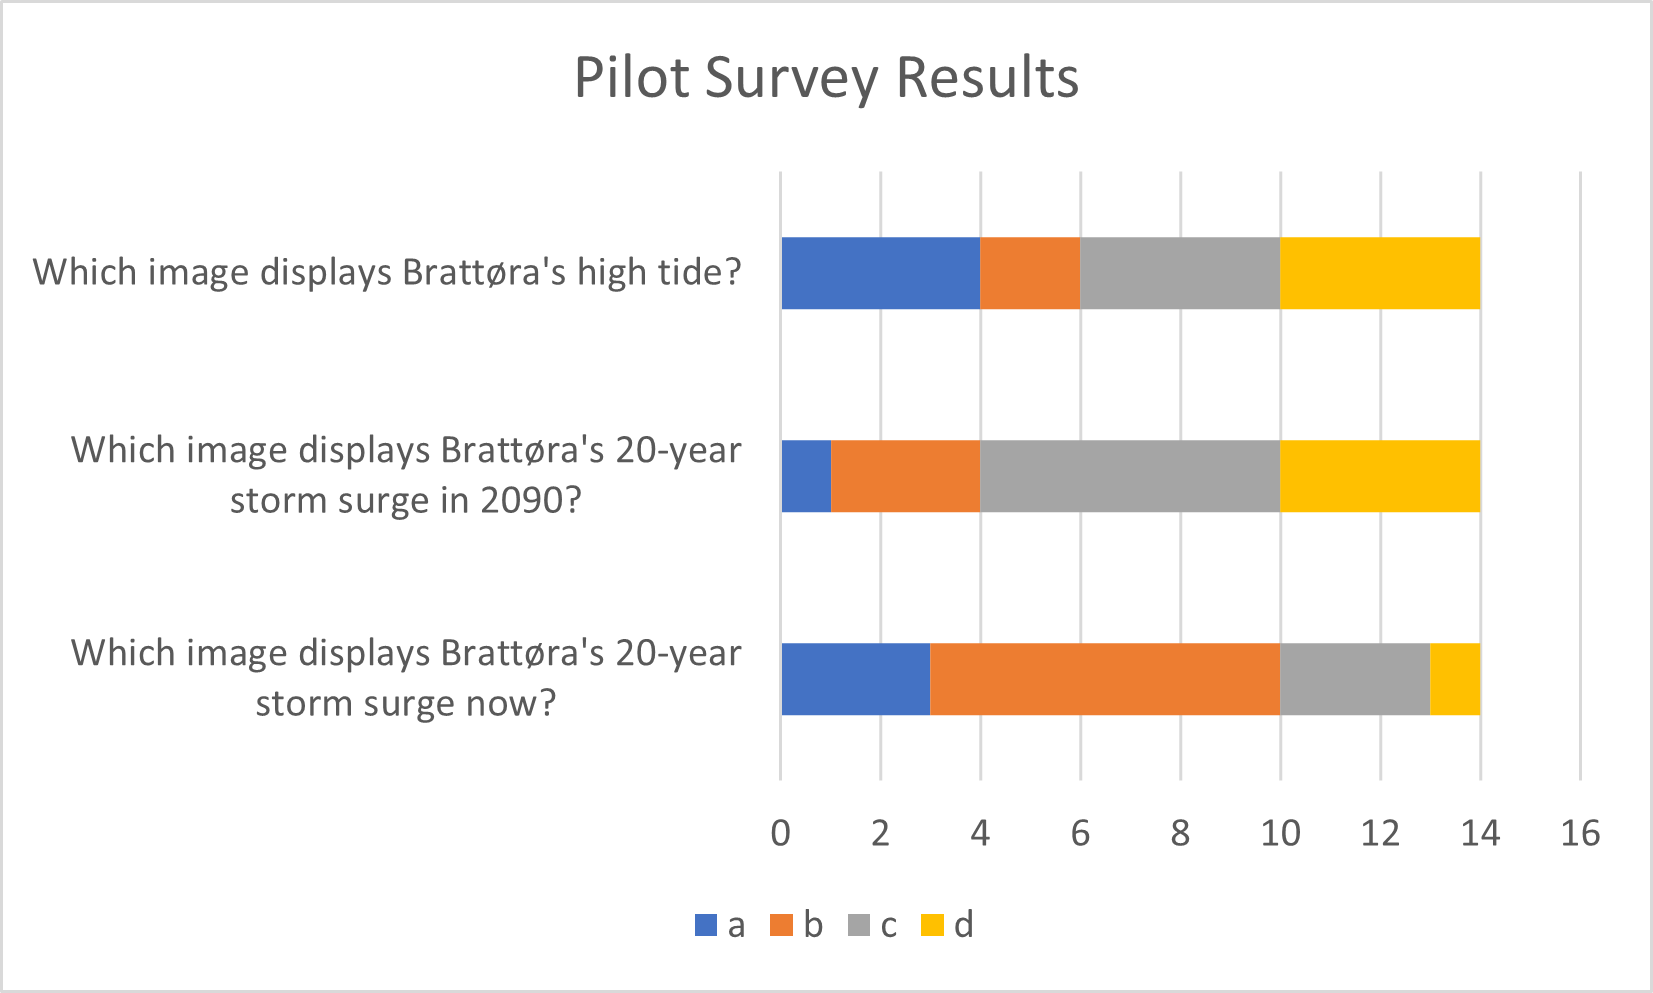
\includegraphics[width=1\textwidth]{fig_results/pilot-survey-results.png}
\begin{frame}{Frame Title}
    Pilot Survey Results - Correct Answers B, B, C
\end{frame}
\paragraph{}

As could be inferred there appears to be no major agreement in results for the pilot survey participants. This could be due to lack of awareness, unlike what was expected but to check a focus group was run. 

\section{Lessons Learned from Focus Group}
Half the participants of the pilot survey were included in the focus group. Several issues with the current survey techniques were highlighted. For ArcGIS survey 123 two participants phones crashed and others highlighted the large amount of mobile data needed to access and fill in the survey as an issue. Furthermore, participants using laptops and smartphones found that the results reflected the machines sensitivity and their own drawing ability more than their awareness to the questions answered. For Nettskjema participants highlighted the difficulty of telling the maps pictured apart. This is reflected in the results of the survey as shown in figure*, above.

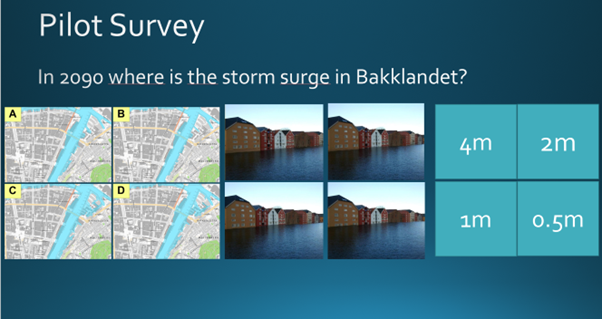
\includegraphics[width=1\textwidth]{fig_results/slide shown in focus group.png}

\paragraph{}
The focus group were then shown other potential methods of gathering awareness using online survey using a slide show with the slide shown above. A limited number were in favour of numbers with the majority favouring the simulated water levels. To avoid the same issues of lack of ability to discussion the pictures and give context to the numbers a combination of simulated pictures plus numbers were chosen. 
The focus group highlighted that Nettskjema was much more trusted than arcgis survey 123 as well. However the main reason for choosing Nettskjema over arcgis survey 123 is that Nettskjema allowed for the input of more images including having images stored on another site allowing for less data to be used to access and complete the survey. Furthermore the new design is better suited for individuals with sight impairments.   
%hmm the two section above may be better suited either in methods or results
%or should rewrite to make it sound more discussiony

\section{Pilot Survey and Focus Group Impacts to Project}
One benefit which is missing when choosing to utilise simulated pictures of water rise rather than maps is that maps better show the area impacted. By looking from a bird’s eye view the scale and wide reach of sea level extremes impact is more obvious. However, this viewpoint is not the view which is normally experienced by those situated within these places. On the other hand, using simulated images allows for the interpretation to be easier and to potentially have more personal/emotional impact as it is closer to the participants lived experiences *need reference*. It is easier to look at a picture and realise that is where the water is in comparison to me, to the places I know rather than the distancing aspect a map has. However, this is only possible with a certain level of realness with the simulated image. Image editing is a slow process, particularly when aiming for realism, for this reason a full explanation of how the simulated images were created is given  in the appendix. 

When redesigning the survey after the Pilot Survey and Focus Group a greater focus was made on making sure the final survey was as accessible as possible. The new survey was tested on several participants before it was shared wider. The time taken to complete the new survey was measure on four participants, including those with mild visual impairments and dyslexia and those who were not using their native tongue. Each of these participants took under six minutes to complete the survey, hence fullfilling the design choice that the majority should be able to complete the survey in under five minutes. 

After this the first group who got access to the survey upon opening to the public were test engineers. This group was targeted to allow errors to be quickly noticed and fixed before the final results were impacted. The first 15 participants had access to 8 surveys, one of which included a typo. Furthermore a link to the survey from the Norwegian website was faulty, preventing this group for filling in surveys on Grillstad. Secondly the option of choosing "utddanning" (formal education) as where you learned about climate change was missing from two of the surveys. These errors were quickly remedied and a maximum of 5 percent of subjects could have been impacted. 

\paragraph{}
It is unlikely considering who the original subjects were that the small errors and typos affected the final results. However there could be a small impact on the variable "info-climate-edu", which in turn impacts the variable "info-climate-sum". The is was deemed to affect a small enough percentage and to be unlikely and so is not considered further.



\section{Survey Considerations}

First getting participants to draw on maps using arcgis survey123 was considered. After the author tried to answer the question on several machines (computer, tablet, 3 different mobiles, paper) it was realised that this technique was too heavily influenced by the subjects drawing ability and the general useability of the machine or technology used to answer the question. For this reason this technique was decided against.
Using just numerical values was decided against due to understanding that these numerical values did not connect well to reality for many participants. What does a storm surge of 1m mean in this area is hard to conceptualise. This left potential subjects guessing answers rather than applying their own awareness/perception/knowledge of sea levels in the chosen areas. Numerical values could be useful for extracting awareness level for those with more professional interests.
\paragraph{}

Next creating 4 maps which showed potential levels of water rise and then asking the subject to answer which was the correct water level was trialled. These maps were made using data from kvartverket and dsb. *would show example question*
This technique was used in a pilot study with a focus group of individuals with high levels of interest in the sea or natural land management. The awareness level of sea level extremes in these individuals could be ranked as high or quite high, but they struggled to answer the trial survey. Especially when using mobiles rather than desktops. Several felt that with enough time they may be able to work it out, but found the differences between the images hard to perceive/spot. Issues with those with poorer eyesight (key stakeholder group is longterm residents so this may be an issue) struggling to distinguish these maps were highlighted.
\paragraph{}

This group were then shown fast mock ups of digitally altered pictures of one of the chosen areas. They felt this was much easier to distinguish, even if it did not show the area of impact to the same extent as the maps. 
After the pilot trial using images altered to show projected levels of sea level extremes was chosen. These images would be complemented with numerical representations. 


\section{Demographics}
The purpose of this research is to assist in the creation of a framework to determine resilience of a place, specifically to sea level extremes. This is to allow repeated measurements of resilience to determine whether a place is making improvements in its resilience. How resilience is improved is done through many techniques including......

Resilience and vulnerability are impacted by demographic variables \cite{rod_integrated_2012}, but improving of resilience shouldn't be done by changing population demographics. Arguing a place is resilient simply due to their being a high percentage of women, or immigrants, or the age of the population is not a use full nor moral lens in which to discuss improvements to resilience. It can be useful to highlight areas or groups who are particularly vulnerable, but not forcing those groups to disperse against their will. For this reason standard demographic questions were not part of this survey. Subjects attributes which local governance could reasonably, cost effectively and most importantly morally impact were prioritised as research variables over demographics. 

Furthermore by asking questions upon gender and age can influence how subjects answer these questions.*citation needed*

Awareness or a hazard is not determined by gender, even if gender can correlate with it.  Gender was determined not a key variable from literature review before the creation of the survey. This is the same for the majority of demographic variables which were not investigated during this research.

Certain demographic questions can be answered by inferring from the results to key questions. For example language skills and even immigration status can be inferred from the subjects decision to complete the survey in Norwegian or English. The lack of availability of the survey in other languages is a limiting factor. Percentage of the population who do not have a reasonable understanding of either Norwegian or English in Trondheim is ****. For this reason plus limitations of funds, researcher skills and time it was deemed acceptable for the posters, emails, social media, website and surveys to only be available in Norwegian and English. However, if this was to be repeated in other locations or nationally this would need to be reconsidered. 

The key demographic that was considered was interest level and professional experience with sea level extremes. ***** highlights that those with professional experience of the relevant hazard or have professional interest are more aware and hence improve an places resilience to the specific hazard. Unfortunately even with an extended deadline marine workers were not an included part of this research. There is a small percentage who have professional interest in sea level extremes see table** below. 

\begin{table}[!ht]
    \centering
    \begin{tabular}{|l|l|l|l|l|l|}
    \hline
       & Not & Low & Medium & High & Professional \\ \hline
       code & 1 & 2 & 3 & 4 & 5 \\ \hline
        No. Respondents & 8 & 22 & 71 & 40 & 12 \\ \hline
    \end{tabular}
    \caption{Interest Level of Subjects in Sea Level Extremes}
    \label{interest_level_table}
\end{table}

As can be seen above the majority have medium level interest in sea level extremes. The spread of results to this question is approximatley normal, which could be seen as either that a good spread of subjects were contacted. However whether this does correctly model Trondheim's population level of interest in the subject is not very likely.  Survey participants were self selecting so that subjects have volunteered their time even with low or no interest in the research is helpful, but it is to be expected that people with an interest in a subject are more likely to take part in a survey.

This has been attempted to be minimised by making the survey as short and as easy to do as possible and by utilizing the researchers network. For more discussion on the careful utilisation of the researchers network to reach subjects who could have been missed find it under the section Survey Access. 

\section{Citizen Science}
Reference: Robinson et al (2012) Guide to citizen science: developing, implementing and evaluating citizen science to study biodiversity and the environment in the UK 
Why citizen science key for this project?
•	Resilience is assumed to be dependent on knowledge/awareness of potential population impacted by disaster/event
•	By including citizens and making them start to think about changing resilience of place to SLE’s may actually improve resilience
•	Need to consider a broad sector of societies awareness
•	Results driven by societal need (as highlighted by UN SDGs) hence moral allowance / legitimacy to ask for help / peoples time

The decision to utilise citizen science is driven by societal need, specifically whether this fulfils policy needs or community needs. for the reasons outlined in the introduction researching resilience to SLE requires knowledge of the awareness that the population has of the risk/vulnerability. Furthermore the gathering of this information has the potential to positively impact the resilience level by improving the awareness of the mentioned vulnerability. 

\section{Survey Access}

\begin{table}[!ht]
    \centering
    \begin{tabular}{|l|l|l|l|l|l|l|}
    \hline
     Access type & poster & email & social & via organisation  & via place of  & personal connection \\ \newline
       &  & & media & n membership & employment & to researcher \\ \hline
       code & 1 & 2 & 3 & 4 & 5 & 6 \\ \hline
      No. Respondents & 70 & 2 & 48 & 2 & 4 & 24 \\ \hline
    \end{tabular}
      \caption{Access to Survey}
      \label{access_survey}
\end{table}

\section{Future Research}
•	Send emails earlier
o	Possibly change that up a bit too
•	Posters seem to work – for ongoing project consider budget here
•	If time /budget allowed having a way of connecting where the poster is to the participants response could be interesting
•	This proved difficult without having different qr code /link on each poster so was ignored due to budget constraints / too much effort

\section{Summary of Discussion of Framework - Lessons Learned}
%target marine workers earlier in process
%posters seem to be best method of accessing, followed by social media
%accessing at different season may impact results
%improve question phrasing so people dont just tick one box


The likelihood of their being another sea level extreme event in Trondheim before anyone gets the chance to repeat this research is significant. If this research was to be repeated it would be important to add any new sea level extreme events to the question on do you remember these events. 